\chapter{Methodology}
\label{chap:met}

This chapter describes the research methodology used to investigate whether software maintainability can be improved through the implementation of architectural tactics using a Large Language Model (LLM). The methodology defines the research design, experimental pipeline, dataset preparation, maintainability measurement approach, LLM-based improvement process, experimental procedure, and evaluation method.

\section{Research Design}

This study follows an experimental research design aimed at evaluating the effect of LLM-assisted architectural improvements on software maintainability. The experiment is based on a pre-test/post-test design, in which maintainability metrics are measured before and after the application of architectural tactics.

The independent variable in this experiment is the application of architectural tactics implemented with the assistance of a Large Language Model.

The dependent variable is software maintainability, measured using quantitative static analysis metrics, primarily the Maintainability Index (MI), as well as architectural and documentation-related indicators.

The experiment was conducted on a dataset of real-world open-source Python backend repositories. Each repository was analyzed in its original state, then modified using LLM-guided architectural improvements, and analyzed again. The difference between the initial and final maintainability metrics was used to assess the effectiveness of the approach.

This research design enables an objective evaluation of whether LLM-assisted architectural tactic implementation can produce measurable improvements in maintainability.

\section{Experiment Overview}

The experiment was implemented as an automated pipeline consisting of sequential stages applied to each repository in the dataset. The pipeline ensures consistent processing and reproducibility of the results.

The overall experimental pipeline consists of the following stages:

\begin{enumerate}
\item Repository clone
\item Static analysis BEFORE improvement
\item Architecture detection
\item Tactic selection
\item Tactic implementation
\item Static analysis AFTER improvement
\end{enumerate}

The overall experimental pipeline is illustrated in Figure \ref{fig:pipeline}.

\begin{figure}[H]
\centering
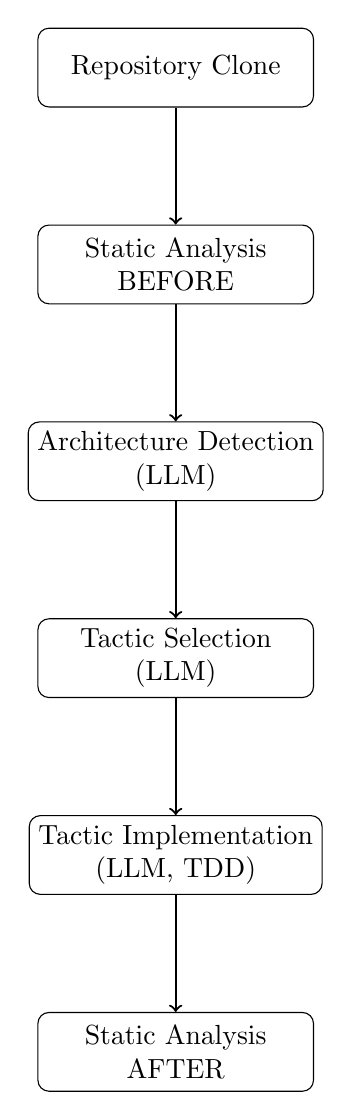
\begin{tikzpicture}[
node distance=2.5cm,
every node/.style={
draw,
rectangle,
rounded corners,
minimum width=3.5cm,
minimum height=1cm,
align=center
},
arrow/.style={
->,
thick
}
]

\node (selection) {Repository Clone};

\node (before) [below of=selection]
{Static Analysis \\ BEFORE};

\node (architecture) [below of=before]
{Architecture Detection \\ (LLM)};

\node (tactic) [below of=architecture]
{Tactic Selection \\ (LLM)};

\node (implementation) [below of=tactic]
{Tactic Implementation \\ (LLM, TDD)};

\node (after) [below of=implementation]
{Static Analysis \\ AFTER};


\draw[arrow] (selection) -- (before);
\draw[arrow] (before) -- (architecture);
\draw[arrow] (architecture) -- (tactic);
\draw[arrow] (tactic) -- (implementation);
\draw[arrow] (implementation) -- (after);

\end{tikzpicture}
\caption{Experimental pipeline for LLM-based architectural maintainability improvement}
\label{fig:pipeline}
\end{figure}

Each stage is described below.

\textbf{Repository clone}

Repositories were collected and filtered to obtain a dataset of Python backend systems suitable for architectural analysis and modification.

\textbf{Static analysis BEFORE improvement}

Static analysis was performed on each repository to calculate baseline maintainability metrics.

\textbf{Architecture detection}

The LLM analyzed the repository structure and source code to identify the current software architecture.

\textbf{Tactic selection}

Based on the detected architecture and maintainability issues, the LLM selected an appropriate architectural tactic from a predefined catalog.

\textbf{Tactic implementation}

The LLM implemented the selected tactic using a Test-Driven Development (TDD) approach to ensure correctness and minimize unintended side effects.

\textbf{Static analysis AFTER improvement}

After implementation, static analysis was performed again to measure maintainability metrics.

\section{Dataset Preparation}

The dataset used in this experiment consists of open-source Python backend repositories collected from GitHub.

Dataset preparation was performed using a multi-stage automated filtering process.

First, repository metadata was collected from multiple CSV files containing candidate repositories. These datasets were merged, and duplicate repositories were removed based on their unique full names. For each repository, additional metadata, including the number of GitHub stars, was retrieved using the GitHub REST API. The number of stars was used as an indicator of repository relevance and activity.

Next, repositories were filtered to select backend-oriented Python systems. Each repository was cloned locally and analyzed. The following inclusion criteria were applied:

\begin{itemize}
\item Presence of a requirements.txt file, indicating a Python dependency-based backend project
\item Presence of Python source files
\item Absence of Machine Learning dependencies such as torch, tensorflow, scikit-learn, keras, transformers, and similar libraries
\item Absence of directories typically associated with experimental or non-production code, such as notebooks, experiments, examples, ml, or ai
\end{itemize}

These filtering criteria ensured that the dataset consisted of backend-oriented Python software systems suitable for architectural analysis and maintainability improvement.

Finally, static analysis was performed on each repository to collect initial maintainability metrics, which were included in the dataset.

\section{Maintainability Measurement}

Software maintainability was evaluated using static code analysis metrics. The primary metric used in this experiment was the Maintainability Index, supplemented by architectural and documentation metrics.

\subsection{Maintainability Index}

The Maintainability Index is a composite metric designed to estimate the maintainability of software based on code complexity and size characteristics.

The Maintainability Index was calculated using the Radon static analysis tool.

Radon computes the Maintainability Index based on:

\begin{itemize}
\item Cyclomatic complexity
\item Lines of code
\item Halstead Volume
\end{itemize}

The Maintainability Index provides a numeric value, typically ranging from 0 to 100, where higher values indicate better maintainability.

For each repository, the average Maintainability Index across all analyzed files (MI\_avg) was used as the primary maintainability indicator.

\subsection{Architectural Metrics}

In addition to the Maintainability Index, architectural metrics were collected to assess structural maintainability.

These metrics include:

\begin{itemize}
\item Number of packages
\item Average fan-out
\end{itemize}

These metrics provide insight into modularity, coupling, and architectural complexity.

Higher coupling and fan-out generally indicate lower maintainability.

\subsection{Documentation Metrics}

Documentation quality also affects maintainability.

The following documentation metrics were collected:

\begin{itemize}
\item Docstring coverage
\item Presence of README file
\end{itemize}

Docstring coverage measures the proportion of documented code elements.

Repositories with better documentation are generally easier to maintain.

\section{LLM-based Architecture Improvement}

Architectural improvement was performed using a Large Language Model.

The LLM was used in three stages:

\begin{enumerate}
\item Architecture detection
\item Tactic selection
\item Tactic implementation
\end{enumerate}

\subsection{Architecture Detection}

The LLM analyzed the repository structure and source code to identify architectural characteristics.

The analysis included:

\begin{itemize}
\item File structure
\item Module organization
\item Imports and dependencies
\end{itemize}

Based on this information, the LLM produced a structured description of the repository architecture.

\subsection{Tactic Selection}

After detecting the architecture and analyzing maintainability issues, the LLM selected an appropriate architectural tactic from a predefined catalog of architectural tactics.

Architectural tactics represent design decisions aimed at improving specific quality attributes, including maintainability.

The LLM selected the tactic expected to produce the greatest maintainability improvement while considering trade-offs and risks.

\subsection{Tactic Implementation}

The selected architectural tactic was implemented by the LLM using a Test-Driven Development approach.

The implementation process followed these steps:

\begin{itemize}
\item Creation of a failing test describing the desired behavior
\item Implementation of minimal code required to pass the test
\item Iterative refinement
\end{itemize}

This approach ensured correctness and minimized unintended modifications.

The implementation was constrained to avoid unrelated modifications.

\section{Experimental Procedure}

The experiment was executed using an automated pipeline.

For each repository, the following procedure was performed:

\begin{enumerate}
\item The repository was cloned locally
\item Static analysis was performed to calculate baseline maintainability metrics
\item The LLM analyzed the repository and detected its architecture
\item The LLM selected an appropriate architectural tactic
\item The LLM implemented the tactic
\item Static analysis was performed again after implementation
\item Maintainability metrics before and after improvement were recorded
\item The repository was removed from the local environment
\end{enumerate}

This procedure ensured consistent and isolated processing.

\section{Evaluation Method}

The effectiveness of the architectural improvements was evaluated by comparing maintainability metrics before and after LLM-based modification.

The primary evaluation metric was the change in Maintainability Index.

Maintainability improvement was calculated as:

\begin{equation}
Improvement = MI_{after} - MI_{before}
\end{equation}

Positive values indicate improved maintainability.

Negative values indicate reduced maintainability.

In addition to Maintainability Index, changes in architectural and documentation metrics were also analyzed.

The results were aggregated across all repositories to evaluate overall effectiveness.

This evaluation method provides a quantitative basis for assessing whether LLM-assisted architectural tactic implementation improves software maintainability.
